\section{Jatkotutkimusaiheita}

Luvussa \ref{tulokset} selvisi, että pistedatan kompressoiminen johtaa pienempien tiedostokokojen lisäksi myös oktettipuun rakentamisen nopeutumiseen. Toisaalta kompression purkaminen vie runsaasti laskenta-aikaa renderöintivaiheessa. Laitossuunnitteluohjelmistossa tallennustilan tehokas käyttö ja pistepilven saaminen nopeasti katsottavaksi ovat tärkeää, joten olisi syytä tutkia, saadaanko kompression purkamista nopeutettua. Yksi mahdollisuus olisi säikeistää pisteiden lataamista niin, että yksi säie lukee pisteitä levyltä, toinen purkaa niiden kompressiota ja kolmas kopioi niitä näytönohjaimelle.

Oktettipuun solmujen järjestäminen ruudulle projisoidun koon mukaan vei runsaasti laskenta-aikaa, minkä johdosta luvussa \ref{render} esitetty renderöintialgoritmi suoriutui heikosti suoraviivaiseen puskurivirralla renderöintiin verrattuna. Voidaan kuitenkin katsoa renderöidyn pistepilven korkeamman tiheyden kameran lähellä olevan tärkeämpää kuin absoluuttinen pisteiden määrä. Solmujen järjestämistä voisi myös nopeuttaa helposti säikeistämällä renderöintialgortimi niin, että yksi säie valikoi puusta solmuja prioriteettijonoon, josta toinen säie ottaa aina suurimman prioriteetin omaavan solmun renderöitäväksi.

Pistebudjetin käyttö pistepilveä renderöitäessä mahdollistaa interaktiivisen ruudunpäivitysnopeuden, mutta huonontaa renderöidyn kuvan laatua. Kuvassa \ref{lod_border} näkyy ilmanvaihtohuoneen katossa ikäviä tarkkuustasojen eroja. Kun puusta renderöidään solmuja niiden kuvaruudulle projisoidun koon mukaan eikä taso kerrallaan, voi kuvassa esiintyä suuria tiheyseroja. Tiheyseroja voisi vähentää ja kuvan laatua parantaa implementoimalla esimerkiksi Schützin \cite{potree} ehdottaman muokkautuvan pistekoon algoritmin. 

\begin{figure}
    \centering
    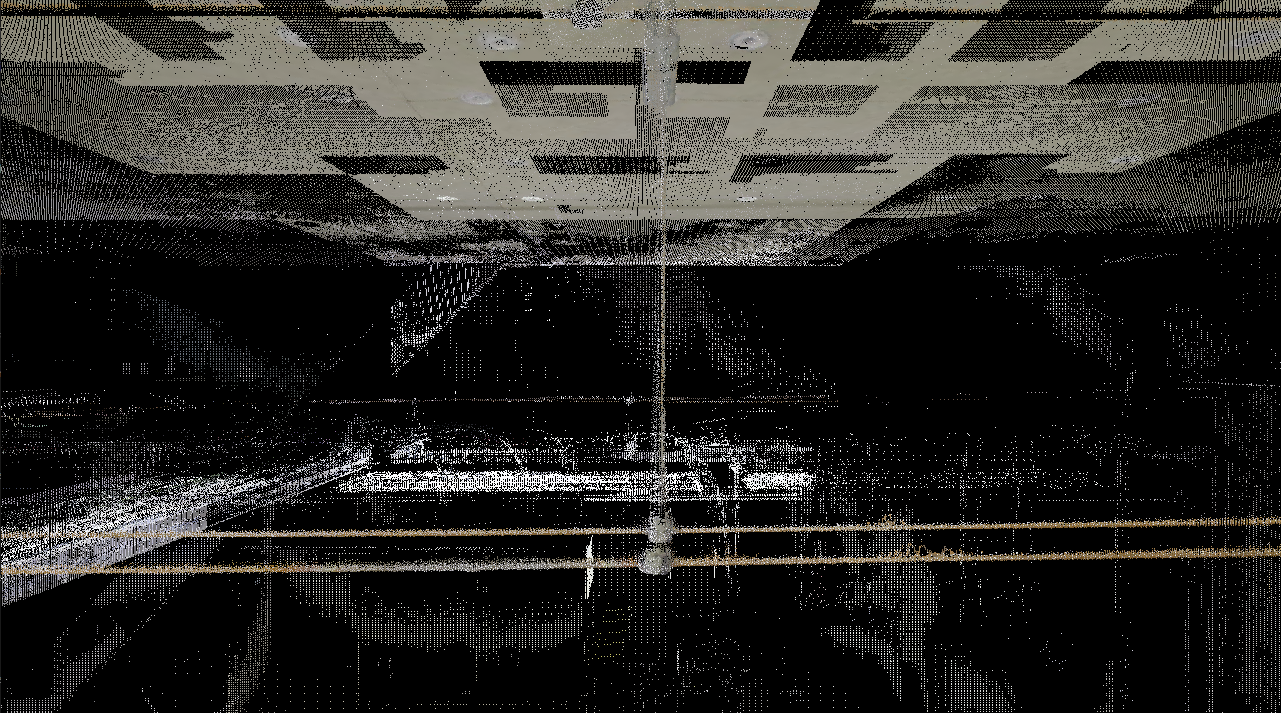
\includegraphics[width=0.7\textwidth]{tuloksia/ilmastointi_2M/ilmastointihuone_vesijohto_overviewbuf.png}
    \caption{Kahden miljoonan pisteen budjetin käyttäminen aiheuttaa ilmanvaihtohuone-pilvessä häiritseviä tarkkuustasojen välisiä eroja.}
    \label{lod_border}
\end{figure}

Laitossuunnitteluohjelmistossa pistepilven renderöintiä voidaan kuitenkin jatkaa monen ruudun ajan, eikä pistebudjetin käyttäminen ole tarpeen. 3d-maisema pistepilvineen ja 2d-grafiikka, kuten kursori ja muut avustimet, voidaan piirtää näytönohjaimelle eri puskureihin. Näin on mahdollista renderöidä uudestaan vain kursori, kun käyttäjä liikuttaa hiirtä, minkä jälkeen pistepilven renderöintiä voidaan jatkaa siitä mihin viimeksi jäätiin. Oktettipuun solmujen järjestäminen tärkeyden mukaan on silti tarpeen. Kuten kuvasta \ref{img:worksite_vertailu} näkyy, järjestämisen ansiosta katselupistettä lähellä olevat mielenkiintoiset alueet tarkentuvat nopeammin.

Mallinnustyössä pistepilvi täytyy usein renderöidä useaan maisemaan. Käytännössä joudutaan harvoin tilanteeseen, jossa kamerat liikkuvat ja pistepilviä joudutaan päivittämään monessa maisemassa samaan aikaan. Kuitenkin olisi suotavaa, jos visualisoija renderöisi ensin pistepilven yleiskuvan jokaiseen maisemaan, minkä jälkeen se kävisi maisemia läpi ja antaisi kullekin pienen aikasiivun pistepilven tarkentamiseen. Samoin usean pistepilven tapauksessa ei saisi käydä niin, että yksi pilvi piirretään täyteen tarkkuuteensa ennenkuin toista on edes aloitettu. 

